% directive: sckaOverviewFigure
% aria-label: One epoch of an SCKA built from a KEM and an erasure code: KEM key generation gives party A the pair (pk, sk); A sends pk to B as erasure-coded chunks, some of which the adversary drops; B runs Encaps(pk) to obtain (c, k_B) and returns c the same way; A runs Decaps(sk, c) to obtain k_A. Correctness requires k_A = k_B with probability at least 1 - epsilon for every adversary scheduling the deliveries.
\documentclass[tikz,border=6pt]{standalone}
\usepackage[T1]{fontenc}
\usepackage{amsmath,amssymb}
\renewcommand{\familydefault}{\sfdefault}
\usepackage[eulergreek]{sansmath}
\sansmath
\usepackage{xcolor}
\usepackage{tikz}
\usetikzlibrary{positioning,calc,arrows.meta,fit,backgrounds,decorations.pathreplacing}
\definecolor{commentcolor}{HTML}{666666}
\definecolor{signalblue}{HTML}{3A76F0}
\definecolor{signalgreen}{HTML}{2A7B7B}
\definecolor{signalolive}{HTML}{4E7F60}
\definecolor{signalpurple}{HTML}{6B3FA0}
\definecolor{adversaryred}{HTML}{B42318}
\newcommand{\Encode}{\mathsf{Encode}}
\newcommand{\Decode}{\mathsf{Decode}}
\tikzset{
  panel/.style={draw=gray!45, line width=0.5pt, rounded corners=4pt, fill=gray!3, inner sep=6pt},
  algbox/.style={draw=signalolive!80, line width=0.7pt, rounded corners=3pt, fill=signalolive!10,
    inner sep=6pt, font=\small\sffamily, align=center},
  statebox/.style={draw=signalblue!70, line width=0.65pt, rounded corners=4pt, fill=signalblue!6,
    inner sep=6pt, font=\small\sffamily, align=center},
  keypill/.style={draw=signalpurple!75, line width=0.6pt, rounded corners=7pt, fill=signalpurple!9,
    inner xsep=8pt, inner ysep=4pt, font=\small\sffamily},
  chunk/.style={draw=signalblue!75, line width=0.55pt, rounded corners=2pt, fill=signalblue!9,
    minimum width=0.62cm, minimum height=0.50cm, inner sep=1pt, font=\scriptsize\sffamily},
  chunklost/.style={chunk, draw=gray!45, fill=gray!10, text=gray!55},
  sourcechunk/.style={chunk, draw=signalpurple!70, fill=signalpurple!9},
  goodpill/.style={draw=signalgreen!80, line width=0.65pt, rounded corners=7pt, fill=signalgreen!9,
    inner xsep=8pt, inner ysep=4pt, font=\small\sffamily},
  failpill/.style={draw=adversaryred!75, line width=0.65pt, rounded corners=7pt, fill=adversaryred!7,
    inner xsep=8pt, inner ysep=4pt, font=\small\sffamily},
  flow/.style={->, >=Stealth, line width=0.8pt, black},
  lossy/.style={->, >=Stealth, line width=0.5pt, gray!55, dashed},
  slot/.style={draw=gray!60, line width=0.5pt, minimum width=0.42cm, minimum height=0.42cm, inner sep=0pt},
  slotfull/.style={slot, fill=signalgreen!25, draw=signalgreen!70},
  slotempty/.style={slot, fill=white},
  lbl/.style={font=\small\sffamily, inner sep=2pt},
  slbl/.style={font=\scriptsize\sffamily, inner sep=1.5pt},
  note/.style={font=\scriptsize\sffamily\itshape, text=commentcolor, inner sep=1.5pt},
  theorybox/.style={draw=signalgreen!80, line width=0.8pt, rounded corners=4pt, fill=signalgreen!8,
    inner sep=7pt, font=\small\sffamily, align=center},
  instancebox/.style={draw=signalblue!70, line width=0.7pt, rounded corners=4pt, fill=signalblue!6,
    inner sep=7pt, font=\small\sffamily, align=center},
  instof/.style={->, >=Stealth, line width=0.8pt, black},
  uses/.style={->, >=Stealth, line width=0.7pt, dashed, signalolive},
  ecbox/.style={draw=signalblue!70, line width=0.7pt, rounded corners=3pt, fill=signalblue!7,
    inner sep=6pt, font=\small\sffamily, align=center},
  rolepill/.style={fill=signalgreen, text=white, rounded corners=5pt, inner xsep=9pt, inner ysep=4pt,
    font=\sffamily\bfseries},
  advpill/.style={draw=adversaryred!80, line width=0.7pt, rounded corners=5pt, fill=adversaryred!7,
    text=adversaryred, minimum width=1.05cm, minimum height=0.68cm, inner sep=3pt, font=\normalsize},
  timeline/.style={-, line width=0.6pt, gray!55},
}
\newcommand{\tagsf}[1]{{\scriptsize\sffamily\itshape\textcolor{commentcolor}{#1}}}
\newcommand{\notesf}[1]{{\scriptsize\sffamily\itshape\textcolor{signalpurple}{#1}}}

\begin{document}
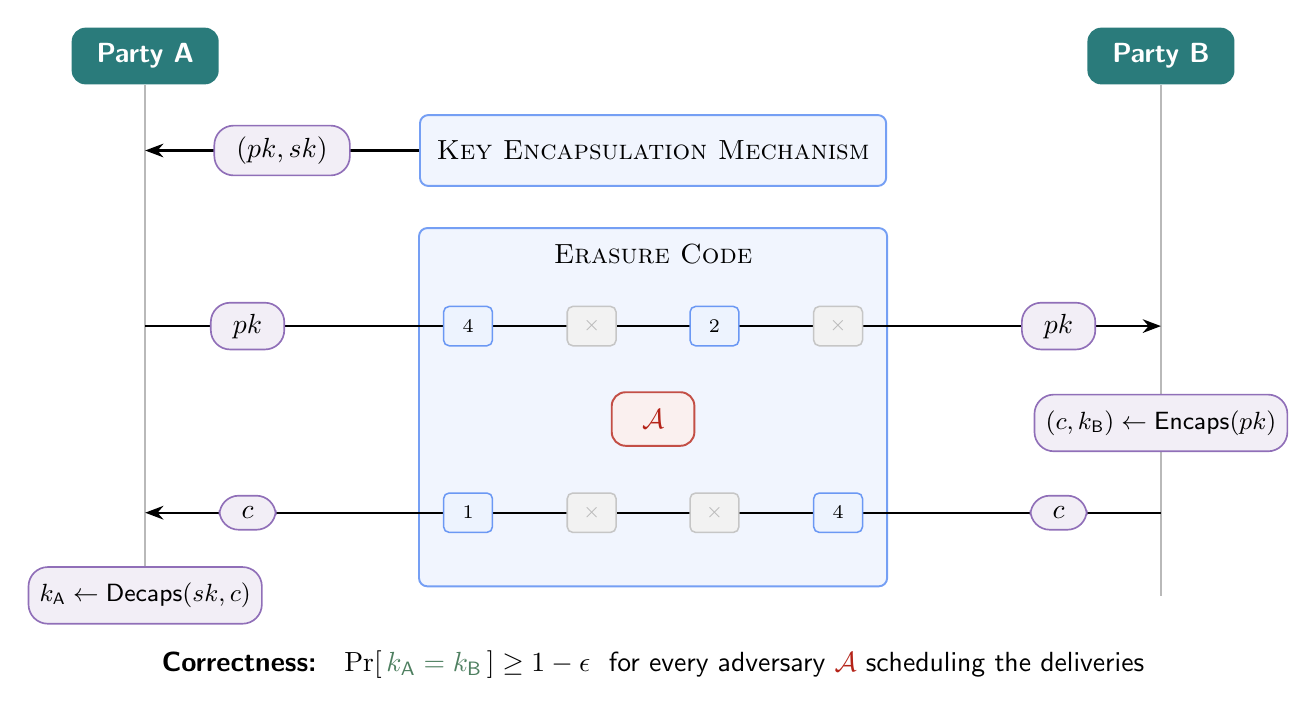
\begin{tikzpicture}[x=1cm,y=1cm]
  \node[rolepill, minimum height=0.72cm] at (-6.45,3.38) (pa) {Party A};
  \node[rolepill, minimum height=0.72cm] at ( 6.45,3.38) (pb) {Party B};
  \draw[timeline] (pa.south) -- (-6.45,-3.48);
  \draw[timeline] (pb.south) -- ( 6.45,-3.48);
  \node[ecbox, minimum width=3.25cm, minimum height=0.90cm, font=\normalsize\sffamily\scshape]
        at (0,2.18) (kem) {Key Encapsulation Mechanism};
  \node[ecbox, fit=(kem), inner sep=0pt, minimum height=4.55cm, yshift=-3.26cm] (ec) {};
  \node[anchor=north, font=\normalsize\sffamily\scshape] at ([yshift=-0.10cm] ec.north) {Erasure Code};
  \coordinate (akeys) at (-6.45,2.18);
  \draw[flow] (kem.west) -- node[midway, keypill, font=\normalsize]
        {$(pk,sk)$} (akeys);
  \coordinate (apk) at (-6.45,-0.05);
  \coordinate (bpk) at (6.45,-0.05);
  \draw[flow] (apk) -- (bpk);
  \node[keypill, font=\normalsize] at (-5.15,-0.05) {$pk$};
  \node[chunk] at (-2.35,-0.05) {$4$};
  \node[chunklost] at (-0.78,-0.05) {$\times$};
  \node[chunk] at (0.78,-0.05) {$2$};
  \node[chunklost] at (2.35,-0.05) {$\times$};
  \node[keypill, font=\normalsize] at (5.15,-0.05) {$pk$};
  \node[advpill] at (0,-1.23) {$\mathcal{A}$};
  \node[keypill, minimum height=0.72cm, inner sep=4pt, font=\small\sffamily] at (6.45,-1.28)
        {$(c,k_{\mathsf B})\gets\mathsf{Encaps}(pk)$};
  \coordinate (act) at (-6.45,-2.42);
  \coordinate (bct) at (6.45,-2.42);
  \draw[flow] (bct) -- (act);
  \node[keypill, font=\normalsize] at (5.15,-2.42) {$c$};
  \node[chunk] at (-2.35,-2.42) {$1$};
  \node[chunklost] at (-0.78,-2.42) {$\times$};
  \node[chunklost] at (0.78,-2.42) {$\times$};
  \node[chunk] at (2.35,-2.42) {$4$};
  \node[keypill, font=\normalsize] at (-5.15,-2.42) {$c$};
  \node[keypill, minimum height=0.72cm, inner sep=4pt, font=\small\sffamily] at (-6.45,-3.47)
        {$k_{\mathsf A}\gets\mathsf{Decaps}(sk,c)$};
  \node[anchor=north, font=\normalsize\sffamily] at (0,-4.05)
        {\textbf{Correctness:}\quad
         $\Pr\!\left[\textcolor{signalolive}{\,k_{\mathsf A}=k_{\mathsf B}\,}\right]\ge 1-\epsilon$
         \ for every adversary \textcolor{adversaryred}{$\mathcal{A}$} scheduling the deliveries};
\end{tikzpicture}
\end{document}
